\subsection{Statusinformationen}
\subsubsection{Ausgangslage}
Die strongSwan Applikation bietet Statusinformation zu aktiven Verbindungen (Child SAs). Diese können über die Vici-Schnittstelle mithilfe der Funktion \textbf{list-sa} unter dem ordered Dictionary \textbf{child-sas} ausgelesen werden. Folgende Einträge sind dabei für uns relevant:
\begin{itemize}
    \item remote-ts
    \item local-ts
    \item bytes-in
    \item bytes-out
    \item packets-in
    \item packets-out
\end{itemize}

\subsubsection{Problematik}
Es stellt sich die Frage, wie dem Webbrowser ständig die aktuellsten Statusinformationen zur Verfügung gestellt werden. 

\subsubsection{Lösungsansatz}
Da die Statusinformationen nur informeller Natur sind, hat die Echtzeit dieser Daten keine hohe Priorität. Somit wurde eine eher triviale Lösung implementiert, die per Ajax Request alle 10 Sekunden die neusten Daten abfragt und darstellt.
\begin{figure}[H]
\centering
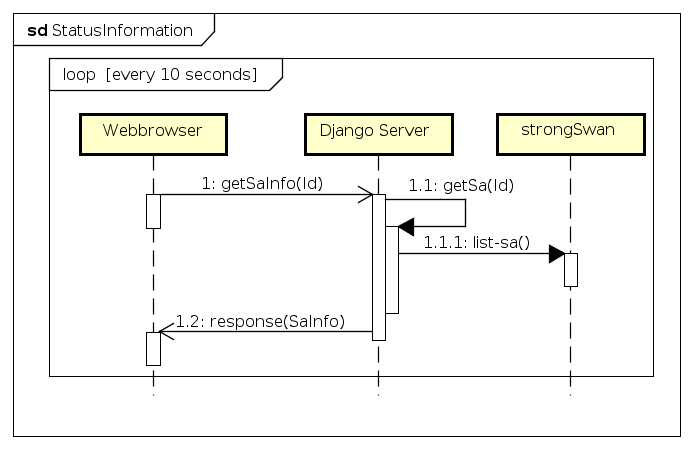
\includegraphics[width=320pt]{images/StatusInformation.png}
\caption[Statusinformationen Sequenzdiagramm]{Statusinformationen Sequenzdiagramm}
\end{figure}

\newpage